\section{Aufbau}
\label{sec:Aufbau}
Im folgenden wird die zylinderförmige KBr-Probe betrachtet, welche sich in einem Rezipienten befindet.
Der Rezipient bildet mit einer Metallplatte, die auf der Probe liegt einen Plattenkondensator.
An diesen angeschlossen sind eine Gleichspannungsquelle und im späteren Verlauf ein Picoamperemeter.
Im Rezipient hersscht außerdem ein Vakuum, um Kondensation von Wasser zu vermeiden.
Zur Temperaturregelung erfolgt über eine Heizspule, die durch ein Netzgerät geregelt werden kann, sowie einen
Kühlfinger aus Kupfer der zur Kühlung in ein Dewar-Gefäß mit Stickstoff gefahren werden kann.
Zum Ablesen der Temperatur befindet sich ein Thermoelement auf dem Boden des Rezipienten.
Der schematische Aufbau des Versuchsaufbaus ist in \autoref{fig:aufbau} dargestellt.
\begin{figure}[H]
    \centering
    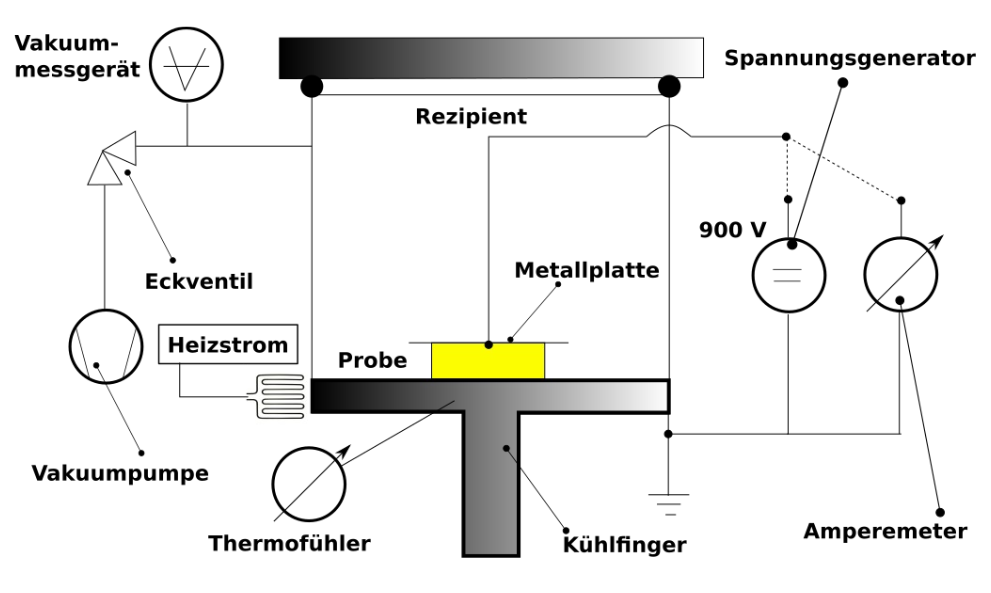
\includegraphics[scale=0.35]{Abbildungen/Skizze.png}
    \caption{Schematischer Aufbau des Versuchs.\cite{V48}}
    \label{fig:aufbau}
\end{figure}


\section{Durchführung}
\label{sec:Durchführung}
Die Probe wird mithilfe der Heizspule auf $T= \qty{320}{\kelvin}$ aufgeheizt. Der Plattenkondensator wird durch Anlegen einer Spannung von
$\qty{950}{\volt}$ aufgeladen um möglichst viele Dipole auszurichten. Dann wird die Probe auf $\qty{210}{\kelvin}$ abgekühlt. Während der Abkühlung
ändert sich die Dipolausrichtung nicht. Wenn die Probe abgekühlt ist, wird das E-Feld abgestellt und der Kondensator wird für $\qty{5}{\minute}$
kurzgeschlossen.
Nun beginnt die Messung.
Während die Heizrate möglichst konstant gehalten wird und $\qty{2}{\kelvin\per\minute}$ nicht übersteigt,
werden die Temperatur und der Depolarisationsstrom in Abhängigkeit von der Zeit aufgenommen.
Während der Messung sollen möglichst wenige Bewegungen gemacht werden um die sensible Strommessung nicht zu beeinflussen.
Die Messung endet wenn die Probe eine Temperatur von circa $\qty{330}{\kelvin}$ erreicht und wird für zwei verschiedene Heizraten durchgeführt.


